%!TEX root = ../../thesis.tex
% https://cyberneticzoo.com/bionics/1957-artificial-muscle-joseph-laws-mckibben-american/
The term \emph{soft robotics} is the abbreviated form of \emph{soft material robotics}. Although the words \emph{soft} and \emph{robotics} have a clear definitions independently, the collocation of the two has sparked vivid discussions in the robotics community for many years -- even touching the territories of the philosophical. Consequently, the exponential scientific interest in soft robotics around 2011 may be seen as a historical cornerstone that has revolutionized our perspective on the branching field of robotics and rekindled its original ambition even before the term \emph{robot} was introduced. Although the debate on the exact terminology is still ongoing, and perhaps may never be closed; we propose a definition for \emph{soft robotics} applicable to this thesis based on an ensemble of prior literature:

\terminology{Soft robotics}{is a robotics subclass with purposefully designed compliant elements embedded into their mechanical structure whose goal is to endow the robot with natural (or biological) motion or compliance.}

The definition above is mostly adopted from Della Santina et al. \cite{}, yet modified to purposefully highlight the importance of soft materials to mimic biological motion -- also referred to as \emph{bio-mimicry}. The ambition of closely mimicking biological creatures is perhaps not often associated with the field of robotics in general, yet the inception of robotics can originally be found in bio-mimicry when regarding its rich history. We would like to implore the reader to embark with us this brief section into the history of (soft) robotics, as to show that the current trends of bio-mimicry in robotics finds roots in a period before classic robotics.
%
\afterpage{
\begin{figure}
\hspace{-7mm}
\includegraphics[width=1.11\textwidth]{./3_chapters/0_introduction/img/timeline.pdf}
\caption{A brief timeline of the state-of-the-art of robotics throughout human history. \textit{(420 BC)} One of the earliest examples of bio-mimicry -- the flying mechanical bird. \textit{(1495)} The Mechanical Knight by Leonardo Da Vinci. \textit{(1738)} Digesting duck patent of Jacques de Vaucanson.  \textit{(1920)} The science-fiction play by Karel \v{C}apek on robots, who introduced the word \emph{robot} into the Oxford English Dictionary originally from his brother Josef \v{C}apek. \textit{(1965)} The first soft robot called Orm designed by V. Scheinman and L. Leifer. \textit{(1968)} The first redundant snake-like robot called Scripps tensor arm patented by V.C Anderson. }
\end{figure}
\clearpage
}

One of the earliest examples of bio-mimicry is a mechanical wooden dove developed by mathematician Archytas of Tarentum in 350 BC. According to historians, the system was driven by compressed air or an internal steam-driven engine to achieve forward propulsion, capable of traveling distances of ~200 \si{\meter} (see note\footnote{It was unclear if the devices was attached to a rope, or autonomous flight was achieved.}). Archytas's invention could be considered as one of the earliest robotic systems -- a machine or device that operates automatically or by remote control -- whose main principles are somewhat analogous to nowadays \emph{drone} technology.  A millennium later, in the period of the High Renaissance, Leonardo da Vinci designed and constructed a mechanical knight around the 1490's. Such mechanical constructions were perhaps closer to conventional rigid robotics given our current robotics perspective. It is well-known that his work was built upon extensive anatomical research, which may have facilitated a deep understanding of the human body into the mechanical knight's robotic design.

\par In the 1920's, shortly after the second industrial revolution (1870 - 1914) and the first world war (1914), the first usage of the work \emph{robot} appeared -- originally meaning 'forced labor by serfs' (\ie, peasants) derived from the Czech word \emph{robota}. An common misconception is that robot implies slave, nonetheless, its origin is somewhat related. The word was popularized by Karel \v{C}apek in his play R.U.R. (Rossum’s Universal Robots) that involves an inventor named Rossum who discovers the secret of creating human-like machines. In his play, Rossom's robots assisted or fully alleviated mankind from any labor. Through human's ambition to assimilate man and machine, the robots ultimately gained the capacity for emotions. Shortly after, the robots, who were created to serve humans, have come to dominate mankind completely. The word \emph{robotics} was later solidified by Isaac Asimov, adapting the term from \v{C}apek. These works of science fiction are perhaps the fundamental groundwork of modern robotics which have led to the base practices of robotics and its corresponding academic field.

Only three decades later, in the 1950's, the first robotic arm called the 'Unimate' was employed in industry. The robot was used for manipulating metal die-casts and welding these to welding these to the main body of automobiles. Interestingly, the robot explored both electric as hydraulic-mechanical actuation, similar to nowadays popular Atlas robot (2013) by the company Boston Dynamics. Note that these robots were still controlled remotely, and rudimentary levels of closed-loop control were applied then. The 1950's also brought forth the McKibben actuators developed by Joseph Laws McKibben -- a well-known work in the field of soft robotics. These McKibben actuator consists of an inflatable inner bladder enveloped with a double-helical weave. When pressurized, the fluidic actuator converted radial expansion into uni-axial contraction since weave inhibited extensive \emph{ballooning} -- a term for undesired radial expansion. The McKibben actuators are perhaps seen as one of the first fundamental technologies that enabled soft robotics and to this day it remains a framework for many soft artificial muscle. Nevertheless, besides fluidics, there exist many other technologies employed in soft robotic motion that predate the invention of the McKibben actuator: such as thermal or chemical expansion/contraction, re-alignment of crystals, di-electric elastomers, magnetism, and naturally electro-mechanical actuation. For instance, the earliest system resambling Dielectric Elastomer Actuators (DEA) were developed W. C. R\"{o}ntgen in 1880. Although these mechanisms do not fall under the class soft robot, they are; however, categorized as soft actuators. We like to emphasize here the difference between soft actuators and soft robots in view of a terminology corresponding with the thesis:
%
\terminology{Soft actuators}{ are controllable flexible components of the constitutive soft robotic system that through external stimuli allow for motion or adaptability of compliance and/or texture.}
%
\noindent The terminology above attempts to address a common ambiguity in the field of soft robotics, that being interchangeably usage the term soft actuator and soft robot.

In 1965, the work of V. Scheinman and L. Leifer proposed a novel pneumatic robot arm named Orm -- the Norwegian word for snake. To the author's knowledge, this pneumatic robot is one of the first soft robots -- and suprisingly the system predates the first rigid redundant snake-like robots (1968). Similar to the anatomy of the snakes, the system featured 28 rubber pneumatic artificial muscle (\ie, bellows) distrubuted along the backbone (\ie, skeletal support) of the robot. The network of artificial muscles were sandwiched between steel plates to prevent disalignment. The soft robotic system could undergo three-dimensional movement by inflation or deflation of embedded pneumatic network, leading to a rich set of movements unseen in earlier robotics. The soft robot can achieve bending in any preferred direction by differential pressurization of each channel, and elongation through synchronized actuation. However, according to \cite{}, the positional accuracy of the system was poor, yet the concept of pneumatically-driven soft arms has continued. Two years later, In 1968, V.C. Anderson developed and patented one of the earliest hyper-redundant robotic manipulators.

% \begin{figure}[t]
% \centering
% \includegraphics[width=0.98\textwidth]{./3_chapters/0_introduction/img/modern_softrobots.png}
% \caption{\textit{a)} Elepant-inspired trunk [14]. \textit{b)}, Fish-inspired aquatic robot [19]. \textit{c)}, Soft-infalatable human robot arm [13]. \textit{d)}, Concentric-tube hard continuum robot[21]. \textit{e)}, Soft quadruped robot [20]. \textit{f)}. Explosion- driven semi-soft 3D printed robot [22]. }
% \end{figure}

% Perhaps a subtle point in the terminology above, is its mention to biology.
% Although the area of soft robotics has grown exponentially since the early 2010's, the field of soft robotics dates back to the early 60's.

% \begin{figure}
% \centering
% \setlength\figurewidth{0.53\textwidth}
% \setlength\figureheight{0.25\textwidth}
% \input{./3_chapters/0_introduction/img/myfigure.tikz}
% \end{figure}

%\subsection{REF}

The first robotic manipulator arm used in the orbital environment was the Space Shuttle remote manipulator system. It was successfully demonstrated in the STS-2 mission in 1981 and is still operational today.

First soft robot: Victor Scheinman and Larry Leifer developed an air-powered robot arm called Orm, which is the Norwegian word for snake.

\begin{itemize}
  \item . F. Shulte, "The Characteristics of the Mckibben Artificial Muscle", The Application of External Power in Prosthetics and Orthetics, pp. 94-115, 1960.
  \item A. Chen, R. Yin, L. Cao, C. Yuan, H. K. Ding and W. J. Zhang, "Soft robotics: Definition and research issues," 2017 24th International Conference on Mechatronics and Machine Vision in Practice (M2VIP), 2017, pp. 366-370, doi: 10.1109/M2VIP.2017.8267170.
  \item  W. C. R\"{o}ntgen, “Ueber die durch Electricität bewirkten Form—und Volumenänderungen von dielectrischen Körpern,” Ann Phys Chem, no. 11, pp. 771-786, 1880.
\end{itemize}
